% Aggregates and figures from results/final-analysis/summary.json
% Source manifest SHA256: 7e885ceecf12a180349369ed9ddfc962ad71f1ea270f68b037a86a396430631d
% Summary SHA256: a181f0840a47c129aeb148f1ea5b36c5941a0943cd5fb1ebfa2acd8bfc28a64c
\newcommand{\FinalAbstractResults}{%
对 3515 个真实学生回合的分析得到任务候选 1010 条、贡献候选 776 条，同回合双维共同非空仅 48 条。秋、春任务候选高阶比例为 19.52\% 与 8.02\%，但把未知回合纳入有界情景后，学期差的符号无法确定。同一 352 回合上，双快严格候选经强复核由 110 条变为 86 条；复核同时产生新候选和撤回候选。356 个有任务候选的学生—学期单元均缺有效 CTQ；完整 AIV 无点分，保守范围揭示了补充过程证据的必要性。
}

\newcommand{\FinalSelectionResults}{%
为量化可判定性对学期比较的影响，固定候选标签，让其余回合的潜在层级在 L1 至 L6 间任取。令总回合为 $N$、候选数为 $n$、候选层级和为 $s$、候选高阶数为 $h$，得到
\begin{equation}\label{eq:unknown}
\mathrm{ABL}_{\rm raw}\in[(s+N-n)/N,(s+6(N-n))/N],\quad
\HOT\in[h/N,(h+N-n)/N].
\end{equation}
这是一种保留候选的条件构造，检查未知部分需要何种约束才能支持总体比较。
\begin{figure}[htbp]\centering
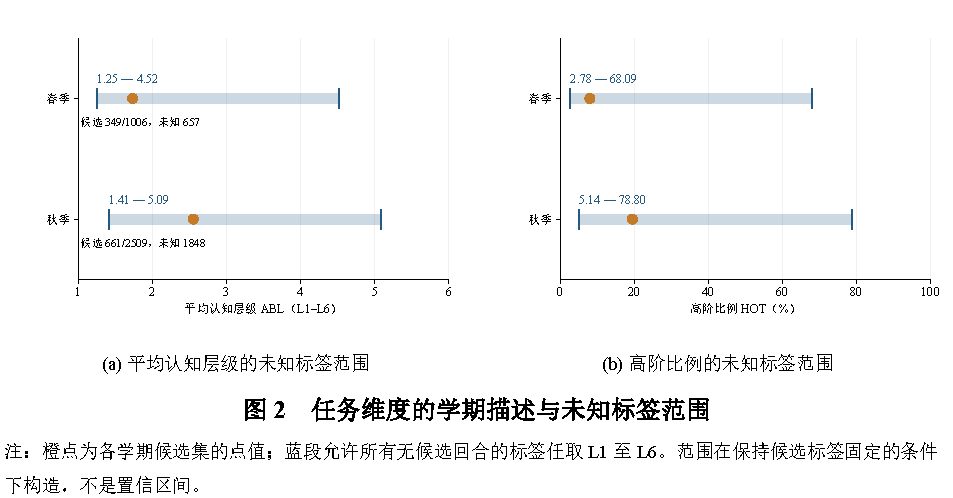
\includegraphics[width=\linewidth,height=.33\textheight,keepaspectratio]{../results/final-analysis/fig03_unknown_labels.pdf}
\caption{任务维度的学期描述与未知标签范围。橙点为各学期候选集；蓝段允许所有无候选回合取 L1 至 L6，范围为条件情景。}\label{fig:unknown}
\end{figure}
秋、春候选任务的平均层级分别为 2.554 与 1.734，高阶占比分别为 19.52\% 与 8.02\%；候选春减秋为 $-11.49$ 个百分点。扩展到全部合格回合后，两学期 HOT 分别在 $[5.14\%,78.80\%]$ 与 $[2.78\%,68.09\%]$ 内，春减秋范围为 $[-76.01,62.95]$ 个百分点。范围覆盖正、负方向，说明已知候选的学期差尚不足以确定总体过程差的方向。贡献维度的春减秋范围同样跨零（$[-80.74,79.10]$ 个百分点），因此后续 B 对两学期保留分层描述。
}

\newcommand{\FinalWorkflowResults}{%
\begin{figure}[htbp]\centering
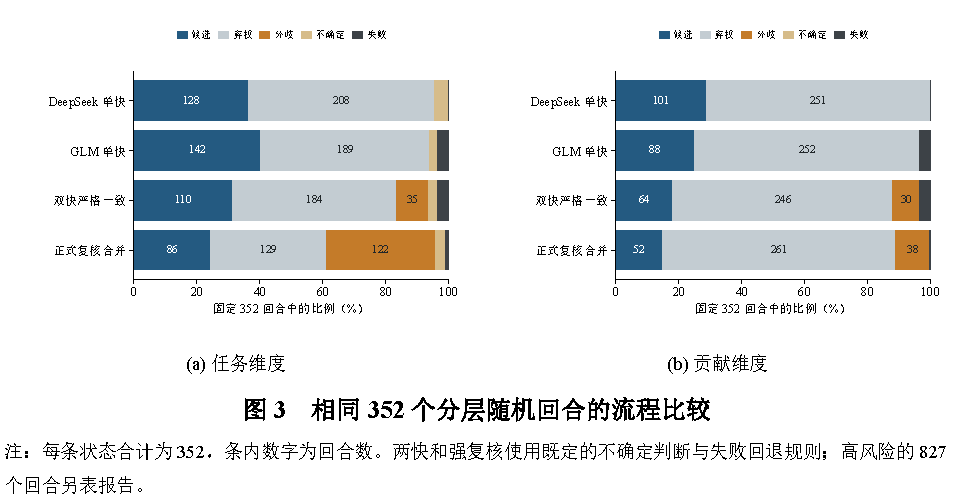
\includegraphics[width=\linewidth,height=.33\textheight,keepaspectratio]{../results/final-analysis/fig02_random_flow.pdf}
\caption{相同 352 个分层随机回合的流程比较。每条状态合计为 352；两快和强复核使用既定的不确定判断与失败回退规则。}\label{fig:flow}
\end{figure}
\begin{table}[htbp]\centering\small
\caption{共同随机集的状态计数；单模型候选不要求另一模型一致}\label{tab:flow}
\begin{tabular}{@{}llrrrrr@{}}\toprule
维度 & 流程 & 候选 & 弃权 & 分歧 & 不确定 & 失败\\\midrule
任务 & DeepSeek 单快 & 128 & 208 & 0 & 16 & 0\\
任务 & GLM 单快 & 142 & 189 & 0 & 9 & 12\\
任务 & 双快严格一致 & 110 & 184 & 35 & 11 & 12\\
任务 & 强复核合并 & 86 & 129 & 122 & 12 & 3\\
贡献 & DeepSeek 单快 & 101 & 251 & 0 & 0 & 0\\
贡献 & GLM 单快 & 88 & 252 & 0 & 0 & 12\\
贡献 & 双快严格一致 & 64 & 246 & 30 & 0 & 12\\
贡献 & 强复核合并 & 52 & 261 & 38 & 0 & 1\\
\bottomrule\end{tabular}
\end{table}
任务候选覆盖由单快的 36.36\%／40.34\%，变为双快严格一致的 31.25\% 和复核合并的 24.43\%。相对双快，复核获得 7 条新候选、撤回 31 条候选；双方都保留候选的 79 条中有 4 条改标。任务分歧由 35 增至 122，表明新增判断使部分原来的一致不再成立。贡献候选由 64 变为 52，获得 13、撤回 25；共同候选 39 条中有 5 条改标。流程选择同时改变覆盖与候选组成，无法用单一候选率评定其准确性。

与随机层相对，827 个风险回合的任务候选由双快的 39 增至复核后的 98，获得 76、撤回 17。风险层包含更集中的初始分歧与失败，复核在这里主要增加可判定结果；随机层则主要减少候选。两种方向共同说明，复核的收益依赖路由所选问题。正文后续指标使用合并后的最终候选，风险层不与随机层合并估计总体误差率。
}

\newcommand{\FinalDistributionResults}{%
\begin{figure}[htbp]\centering
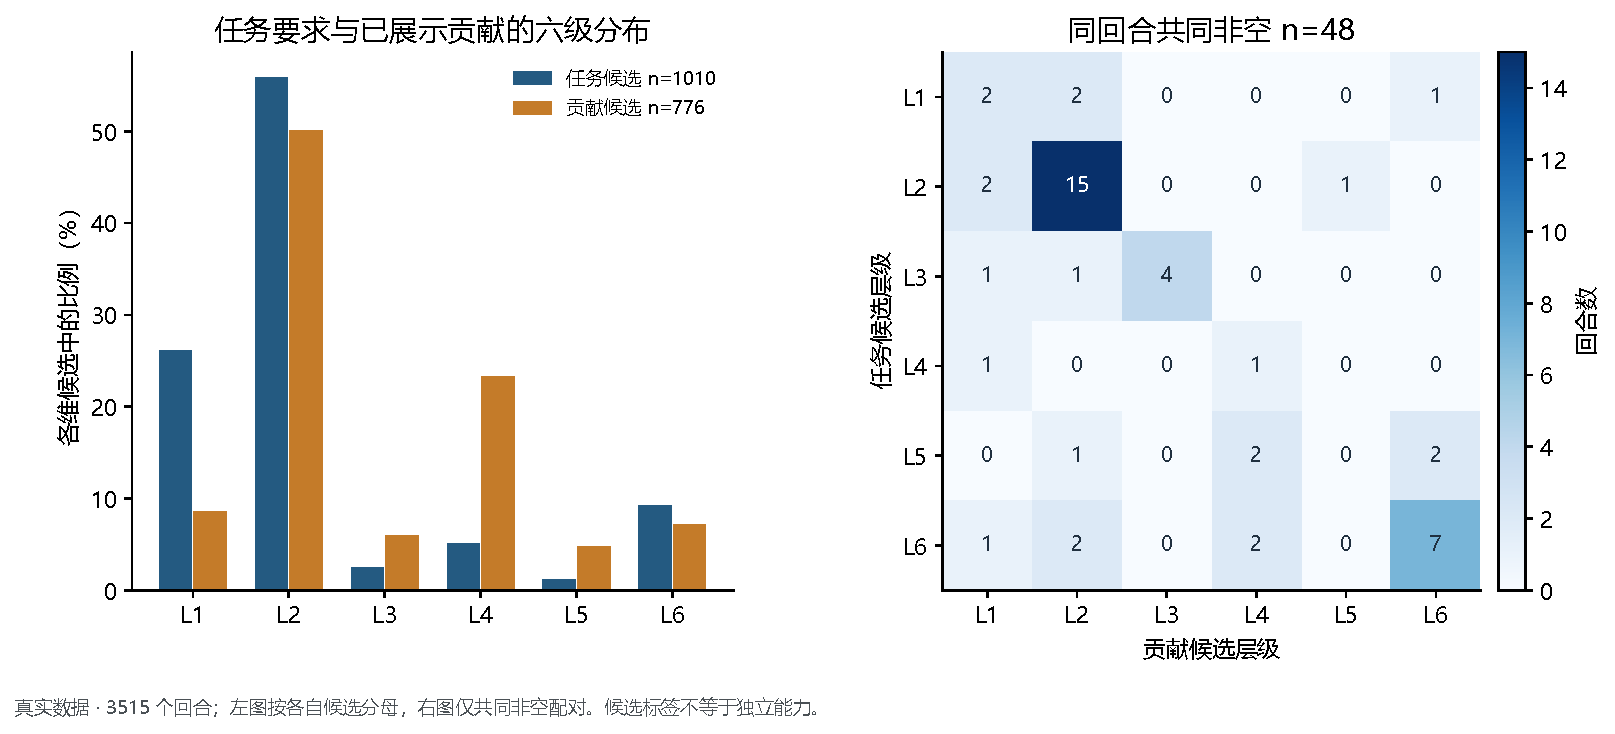
\includegraphics[width=\linewidth,height=.33\textheight,keepaspectratio]{../results/final-analysis/fig01_dimensions.pdf}
\caption{双维边际层级分布与同回合共同非空配对。左图各维按自己的候选分母；右图仅 48 个配对，颜色与数字表示回合数。}\label{fig:dimensions}
\end{figure}
\begin{table}[htbp]\centering\small
\caption{学期内候选描述；学生等权只平均该维至少有一个候选的学生—学期单元}\label{tab:description}
\begin{tabular}{@{}llrrrrr@{}}\toprule
学期 & 维度 & 候选回合 & 候选单元 & 平均层级 & 回合加权 HOT & 学生等权 HOT\\\midrule
秋季 & 任务 & 661 & 257 & 2.554 & 19.52\% & 18.58\%\\
秋季 & 贡献 & 621 & 190 & 2.953 & 37.84\% & 34.29\%\\
春季 & 任务 & 349 & 99 & 1.734 & 8.02\% & 5.56\%\\
春季 & 贡献 & 155 & 54 & 2.542 & 25.16\% & 22.57\%\\
\bottomrule\end{tabular}
\end{table}
任务候选的 L2 占主导；贡献候选则有较多 L4。边际 HOT 分别为 15.54\% 与 35.31\%，但 1010 个任务候选与 776 个贡献候选并非同一组回合，不能据两均值之差推断认知提升。在 48 个同回合共同非空配对中，任务高于贡献 13 个、相同 29 个、低于贡献 6 个，任务减贡献的平均层级差为 0.375；仅 5 个配对满足“任务为 HOT、贡献非 HOT”。共同配对只占全部回合的 1.37\%，支持的是局部双维对应关系。

表\ref{tab:description}同时改变加权单位：秋季任务 HOT 由回合加权 19.52\% 变为学生等权 18.58\%，春季由 8.02\% 变为 5.56\%。方向保持相同，但幅度变化表明较多候选回合的单元对回合加权结果贡献更大。贡献维度也有这种差异。群体报告因此同时呈现候选覆盖、回合统计和学生等权统计，并将“有候选”条件保留到结论中。
}

\newcommand{\FinalHumanResults}{%
\begin{figure}[htbp]\centering
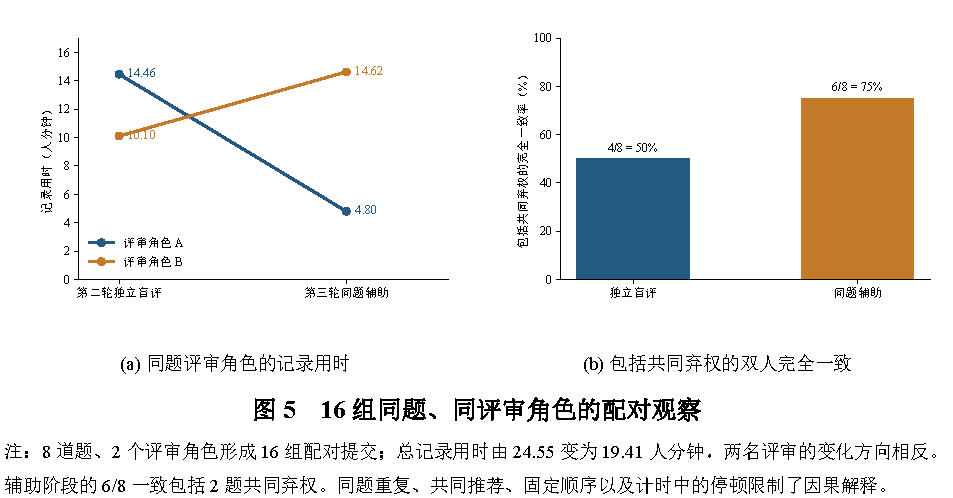
\includegraphics[width=\linewidth,height=.33\textheight,keepaspectratio]{../results/final-analysis/fig04_human_pairs.pdf}
\caption{16 组同题、同评审配对提交。两名评审的记录用时变化方向相反；辅助阶段的 6/8 一致包括 2 题共同弃权。}\label{fig:human}
\end{figure}
评审 A 的记录用时由 14.46 降至 4.80 人分钟，评审 B 由 10.10 升至 14.62 人分钟。合计减少 5.14 人分钟掩盖了个体方向差异；计时还包含停顿，因此保留逐角色数值比只报告一个效率比例更有信息。辅助后的 6 题一致中，4 题给出相同层级、2 题共同弃权，显示校准部分来自对证据不足边界的共同认识。
}

\newcommand{\FinalAssociationResults}{%
资格检查使用 3515 个真实回合，其中 1010 个任务候选；可用逐回合时间戳为 0，严格前瞻关联的合格记录为 0、学生簇为 0。CSV 创建时间虽存在，其语义不支持回合发生顺序；因此本次没有估计回归系数，设计矩阵检查止于样本资格门槛。独立学习结局、无 AI 可比对照和处理前基础也未出现在所分析资料中。
}

\newcommand{\FinalAvailabilityResults}{%
实际学生—学期共 401 个单元，其中 356 个至少有一个任务候选，45 个没有任务候选。候选支持 ABL/HOT/DHI；257 个单元满足 MAB 的字段条件，其余 99 个候选单元位于工具身份缺失的春季。有效会话边尚未核验，CTQ 可计算数为 0，完整 AIV 可计算单元数为 0，点分保持缺失。可计算子指标及缺失原因共同保留。
}

\newcommand{\FinalSensitivityResults}{%
本次求解使用联合可行集的保守外包：将 ABL/HOT/DHI 的单项改标界分别截断至 $[0,1]$，缺失指标取 $[0,1]$，再枚举权重乘子的 32 个顶点。外包保留所有满足改标预算的真实组合，同时可能包含不能共同出现的组合，故其宽度与无法区分比例具有保守性。结果仅针对 356 个有任务候选的学生—学期单元，不外推到 45 个无候选单元。
\begin{figure}[htbp]\centering
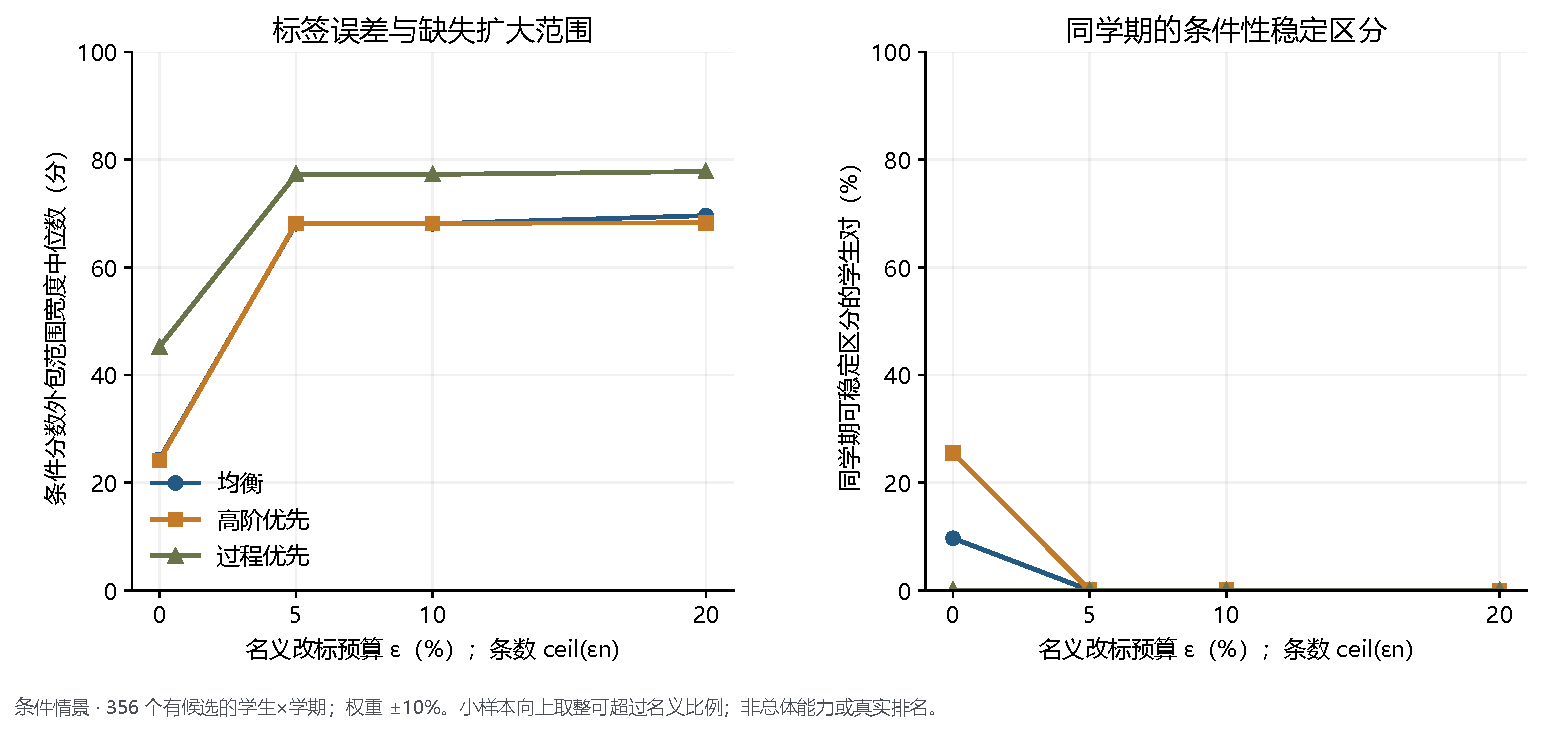
\includegraphics[width=\linewidth,height=.33\textheight,keepaspectratio]{../results/final-analysis/fig05_score_sensitivity.pdf}
\caption{真实候选单元上的条件分数外包范围。权重逐项相对扰动 $\pm10\%$；$\epsilon$ 经向上取整转为改标条数，图中稳定区分限于同学期配对。}\label{fig:sensitivity}
\end{figure}
\begin{table}[htbp]\centering\small
\caption{范围宽度和条件可区分性；356 个候选单元、37747 个同学期对}\label{tab:sensitivity}
\begin{tabular}{@{}rllrr@{}}\toprule
$\epsilon$ & 权重扰动 & 方案 & 宽度中位数（分） & 可稳定区分对数\\\midrule
0.00 & 0\% & 均衡 & 20.00 & 6228/37747\\
0.00 & 0\% & 高阶 & 20.00 & 12575/37747\\
0.00 & 0\% & 过程 & 40.00 & 0/37747\\
0.00 & 10\% & 均衡 & 24.33 & 3651/37747\\
0.00 & 10\% & 高阶 & 24.14 & 9638/37747\\
0.00 & 10\% & 过程 & 45.18 & 0/37747\\
0.05 & 10\% & 均衡 & 68.11 & 0/37747\\
0.05 & 10\% & 高阶 & 68.18 & 1/37747\\
0.05 & 10\% & 过程 & 77.27 & 0/37747\\
0.20 & 10\% & 均衡 & 69.62 & 0/37747\\
0.20 & 10\% & 高阶 & 68.29 & 0/37747\\
0.20 & 10\% & 过程 & 77.81 & 0/37747\\
\bottomrule\end{tabular}
\end{table}
不改标且固定权重时，三方案范围宽度中位数分别为 20、20、40 分；仅加入权重 $\pm10\%$ 扰动后，变为 24.33、24.14、45.18 分。可稳定区分对数分别从 6228、12575、0 降至 3651、9638、0。过程优先给缺失 CTQ 更大权重，因而真实资料不能支持该方案下的稳定区分。

名义 $\epsilon=.05$ 时，$\lceil\epsilon n_i\rceil$ 允许每单元改变 1 至 2 条标签，实际改标比例中位数为 50\%、最大为 100\%；这是候选稀疏条件下的“至少一条改标”检查。加入权重扰动后，三方案外包宽度中位数达到 68.11、68.18、77.27 分，可稳定区分对数为 0、1、0。$\epsilon=.20$ 时三方案均为 0。结果说明，低候选数、结构缺失和外包的保守性共同限制个体分数用途；它不等价于测得了相应比例的标签错误，也不证明所有学生的真实能力相同。
}

\newcommand{\FinalAttackResults}{%
\begin{table}[htbp]\centering\small
\caption{指标攻击与条件反例；均为确定性合成构造}\label{tab:attacks}
\begin{tabularx}{\textwidth}{@{}p{.15\textwidth}p{.30\textwidth}p{.21\textwidth}X@{}}\toprule
对象 & 控制条件与干预 & 数值结果 & 反馈位置\\\midrule
HOT & 标签 $[2,3,4,5]$ 复制一条 L5，保留同一认知内容 & $2/4\to3/5$，增加 0.10 & 依据来源去重，并保留真实重复练习事件\\
MAB & 同一标签，工具数由 1 增至 4 & 均衡分增加 11.39 & C：工具机会与评分权重\\
MAB 对照 & 对上述工具堆叠设 MAB 零权重 & 该攻击增分为 0 & E：同时说明广度激励的取舍\\
DHI & 按预设 $q$ 构造标签分布 & 对称／非对称均为 1 & 依据课程信息设定 $q$，解释限于分布贴合\\\bottomrule
\end{tabularx}
\end{table}
}
